\subsection{半原始模}

定义 4. —— 若一个模是原始子模的一个族的直和，则称它为半原始模。

*例. —— 1) 每个单模都是原始模（VIII，第 45 页）；因此每个半单模都是半原始模（VIII，第 55 页，定义 1）。

\begin{enumerate}
\def\labelenumi{\arabic{enumi})}
\setcounter{enumi}{1}
\tightlist
\item
  若 A 是左诺特环，则每个内射 A-模都是半原始的（X, §1, n° 9, 第 21 页，命题 14 及 X, §1, n° 10, 第 22 页，定理 3, b)）。*
\end{enumerate}

定理 1（阿祖马亚）. —— 设 A 是环，L 是原始 A-模，M 是半原始 A-模。存在唯一的基数，记作 {[}M : L{]}，它具有下列性质：

对 M 作为原始模的直和的每个分解 \(M = \bigoplus_{i \in I} M_i\)，指标 \(i \in I\) 中使 \(M_i\) 同构于 L 的那些指标组成的集合具有基数 {[}M : L{]}。

证明基于下面四个引理。

引理 1. —— 设 M 是一个 A-模，M' 是 M 的一个原始子模，M'\,' 是 M 中与 M' 互补的一个子模。设 u 是 M 的一个自同态。则 u 或 \(1_{M} - u\) 诱导出从 M' 到 M 中与 M'\,' 互补的一个子模的同构。

设 \(p\) 是 M 到 \(M'\) 上的、核为 \(M''\) 的投影，并设 \(v\) 是 \(p \circ u\) 在 \(M'\) 上的限制。先设 \(v\) 是 \(M'\) 的自同构。由于 \(v\) 是单射，\(u\) 在 \(M'\) 上的限制是单射，且我们有 \(u(M') \cap M'' = 0\)。由于 \(v\) 是满射，我们有 \(u(M') \oplus M'' = M\)。因此，\(u\) 诱导出从 \(M'\) 到 M 中与 \(M''\) 互补的一个子模的同构。现在设 \(v\) 不是 \(M'\) 的自同构。则 \(1_{M'} - v\) 是 \(M'\) 的自同构，因为 \(M'\) 是原始模。而 \(1_{M'} - v\) 是 \(p \circ (1_M - u)\) 在 \(M'\) 上的限制。前面的论证表明，\(1_M - u\) 诱导出从 \(M'\) 到 M 中与 \(M''\) 互补的一个子模的同构。

引理 2. —— 设 M 是一个 A-模，它是原始子模的族 \((\mathrm{M}_{i})_{i\in\mathrm{I}}\) 的直和，并设 u 是 M 的一个自同态。对 I 的每个子集 J，令 \(v=1_{M}-u\)，\(M_{J}=\bigoplus_{i\in J}M_{i}\)。则下列两个性质之一成立：

\begin{enumerate}
\def\labelenumi{\alph{enumi})}
\item
  存在一个指标 \(i \in I\)，使 u 诱导出从 \(M_{i}\) 到 M 的一个直因子子模的同构。
\item
  凡 \(J\) 是 \(I\) 的有限子集，\(v\) 都诱导出从 \(M_J\) 到与 \(M_{I-J}\) 互补的一个子模的同构。
\end{enumerate}

若性质 b) 成立，则 v 是单射。

设性质 a) 不成立，我们对 J 的基数用归纳法来确立性质 b)。若 \(J = \varnothing\)，则没有什么要证明的。于是设 J 非空，取 J 的一个元素 i，并令 \(J' = J - \{i\}\)。由归纳假设，v 诱导出从 \(M_{J'}\) 到 M 中与 \(M_{I-J'} = M_{I-J} \oplus M_i\) 互补的一个子模的同构；因此，子模 \(M'' = v(M_{J'}) \oplus M_{I-J}\) 与 \(M_i\) 互补。由引理 1 以及关于 u 的假设，自同态 v 诱导出从 \(M_i\) 到 M 中与 \(M''\) 互补的一个子模的同构；从而 v 诱导出从 \(M_J = M_i \oplus M_{J'}\) 到与 \(M_{I-J}\) 互补的一个子模的同构。

最后的断言来自如下事实：M 是诸子模 \(M_{J}\) 的并，其中 J 取遍 I 的有限子集。

引理 3. —— 设 M 是一个 A-模，它是原始子模的族 \((\mathrm{M}_{i})_{i\in\mathrm{I}}\) 的直和，并设 p 是 M 的一个非零投影算子。存在指标 \(i\in I\)，使 p 诱导出从 \(M_{i}\) 到 \(p(\mathrm{M})\) 的一个直因子子模的同构。

由于 p 非零，\(1_{M} - p\) 不是单射。由引理 2，存在指标 \(i \in I\)，使 p 诱导出从 \(M_{i}\) 到 M 的一个直因子子模的同构。M 的每个以 \(p(\mathrm{M}_{i})\) 为像的投影算子经限制都定义出 \(p(\mathrm{M})\) 的一个以 \(p(\mathrm{M}_{i})\) 为像的投影算子，故 \(p(\mathrm{M}_{i})\) 是 \(p(\mathrm{M})\) 的直因子子模。

引理 4. —— 设 M 是一个 A-模，它是原始子模的族 \((\mathrm{M}_{i})_{i\in\mathrm{I}}\) 的直和，设 L 是一个原始 A-模，并设 N 是 M 的一个直因子子模。设 N 是同构于 L 的子模的族 \((\mathrm{N}_{j})_{j\in\mathrm{J}}\) 的直和，并用 \(I_{L}\) 表示指标 \(i\in I\) 中使 \(M_{i}\) 同构于 L 的那些指标的集合。则有

\[
\operatorname{Card} (\mathrm{J}) \leqslant \operatorname{Card} \left(\mathrm{I} _ {\mathrm{L}}\right).\tag{1}
\]

设 \(N_0\) 是 M 中与 N 互补的一个子模。模 M 是 \(N_0\) 与族 \((N_j)_{j \in J}\) 的直和。对每个 \(j \in J\)，用 \(p_j\) 表示与这一分解相伴的、以 \(N_j\) 为像的 M 的投影算子（II, §1, No.~8, 第 209 页，命题 12）。对每个 \(i \in I\)，用 \(J(i)\) 表示指标 \(j \in J\) 中使 \(p_j\) 诱导出从 \(M_i\) 到 \(N_j\) 的同构的那些指标组成的集合。这个集合是有限的：事实上，若 \(x\) 是 \(M_i\) 的非零元素，且 K 是 J 的有限子集并使 \(x\) 属于 \(\mathrm{N}_0 + \sum_{k\in \mathrm{K}}\mathrm{N}_k\)，则有 \(p_j(x) = 0\) 对一切 \(j\in \mathrm{J} - \mathrm{K}\) 成立，从而 \(\mathrm{J}(i)\) 包含于 \(\mathrm{K}\)。

设 \(j \in J\)。由引理 3，存在指标 \(i \in I\)，使 \(p_j\) 诱导出从 \(M_i\) 到 \(N_j\) 的一个直因子子模的同构。由于 \(M_i\) 非零且 \(N_j\) 是原始的、从而是不可分解的（VIII，第 31 页，命题 4），我们有 \(p_j(M_i) = N_j\)，且 \(j\) 属于 \(J(i)\)。由于模 \(M_i\) 同构于 \(N_j\)、从而同构于 \(L\)，指标 \(i\) 属于 \(I_L\)。这证明 \(J\) 是有限集族 \((J(i))_{i \in I_L}\) 的并。若集合 \(J\) 无限，则集合 \(I_L\) 无限，且我们有（《集合论》，III, §6, No.~3, 第 188 页，推论 3）

\[
\operatorname{Card} (\mathrm{J}) \leqslant \sum_ {i \in \mathrm{I} _ {\mathrm{L}}} \operatorname{Card} (\mathrm{J} (i)) \leqslant \operatorname{Card} (\mathrm{I} _ {\mathrm{L}}).
\]

现在设集合 J 有限，我们对 J 的基数用归纳法证明引理。若 J 为空，则没有什么要证明的。于是设 J 非空，并取 J 的一个元素 j。由前所证，存在指标 \(i \in I_{L}\)，使 \(p_{j}\) 诱导出从 \(M_{i}\) 到 \(N_{j}\) 的同构。令 \(I' = I - \{i\}\)，\(J' = J - \{j\}\)。模 M 是 \(M_{i}\) 与 \(p_{j}\) 的核的直和。它也是 \(M_{i}\) 与子模 \(M' = \oplus_{i' \in I'} M_{i'}\) 的直和。因此，存在（II, §1, No.~9, 第 210 页，命题 13 的推论）一个同构 \(\varphi\)，它把 \(\operatorname{Ker} p_{j} = N_{0} \oplus_{j' \in J'} N_{j'}\) 映到 \(M'\) 。令 \(N' = \varphi\big(\sum_{j' \in J'} N_{j'}\big)\)。子模 \(N'\) 在 \(M'\) 中是一个直因子，且是同构于 L 的原始子模族 \((\varphi(N_{j'}))_{j' \in J'}\) 的直和。把归纳假设应用于 \(M'\) 与 \(N'\)：我们有 \(\text{Card}(J') \leqslant \text{Card}(I_L - \{i\})\)，从而得到不等式 (1)。

我们来证明定理 1。设 \((\mathrm{M}_{i})_{i\in\mathrm{I}}\) 与 \((\mathrm{N}_{j})_{j\in\mathrm{J}}\) 是以 M 为直和的原始子模的两个族。用 \(I_{L}\)（相应地 \(J_{L}\)）表示 \(i\in I\)（相应地 \(j\in J\)）中使 \(M_{i}\)（相应地 \(N_{j}\)）同构于 L 的那些元素的集合。由引理 4，我们有 \(\mathrm{Card}(J_{\mathrm{L}})\leqslant\mathrm{Card}(I_{\mathrm{L}})\)。交换 I 与 J 的角色，即得反向不等式，从而定理得证。

定理 1 中定义的基数 \([M : L]\) 称为 L 在 M 中的原始重数。

推论 1. —— 设 M 与 N 是半原始模。则 M 与 N 同构当且仅当对每个原始模 L 都有 \([M:L]=[N:L]\)。

推论 2. —— 设 M 是一个半原始模。设 \((\mathrm{M}_{i})_{i\in\mathrm{I}}\) 与 \((\mathrm{M}_{j}^{\prime})_{j\in\mathrm{J}}\) 是 M 的原始子模族，使得

\[
\mathrm{M} = \bigoplus_ {i \in \mathrm{I}} \mathrm{M} _ {i} = \bigoplus_ {j \in \mathrm{J}} \mathrm{M} _ {j} ^ {\prime}.
\]

则存在一个自同构 \(u\)（作用于 \(M\)）与一个双射 \(\varphi\)（从 \(I\) 到 \(J\)），使 \(u(M_i) = M_{\varphi(i)}'\) 对每个 \(i \in I\) 成立。

对每个原始模 L，用 \(I_{L}\)（相应地 \(J_{L}\)）表示指标 \(i \in I\)（相应地 \(j \in J\)）中使 \(M_{i}\)（相应地 \(M_{j}'\)）同构于 L 的那些指标的集合。形如 \(I_{L}\)（相应地 \(J_{L}\)）的非空集合构成 I（相应地 J）的一个分拆，且对每个 L，有

\[
\mathrm{Card} (\mathrm {I_ {L}}) = \mathrm{Card} (\mathrm {J_ {L}}) = [ \mathrm{M:L} ];
\]

由此即得该推论。

推论 3. —— 设 M、N、P 是半原始模。设 \(M \oplus P\) 同构于 \(N \oplus P\)，且对每个原始模 L，\([P : L]\) 都有限。则 M 与 N 同构。

按假设，我们有

\[
[ \mathrm{M}: \mathrm{L} ] + [ \mathrm{P}: \mathrm{L} ] = [ \mathrm{N}: \mathrm{L} ] + [ \mathrm{P}: \mathrm{L} ]
\]

对每个原始模 L 成立。由于 \([P:L]\) 有限，由（《集合论》，III, §3, No.~4, 第 162 页，命题 8）并经归纳，可得对每个原始模 L 有 \([M:L]=[N:L]\)。于是由推论 1，模 M 与 N 同构。

推论 4. —— 设 M 与 N 是半原始模。设存在整数 d \textgreater{} 0 使 \(M^{d}\) 同构于 \(N^{d}\)。则模 M 与 N 同构。

设 \(\mathrm{L}\) 是一个原始模。按假设，我们有

\[
d [ \mathrm{M}: \mathrm{L} ] = d [ \mathrm{N}: \mathrm{L} ].
\]

因此有等式 \([M:L]=[N:L]\)：事实上，对每个无限基数 a 有 da = a（《集合论》，III, §6, No.~3, 第 188 页，推论 4）。于是由推论 1，模 M 与 N 同构。

推论 5. —— 设 M 是一个半原始模，它是原始子模的有限族 \((\mathrm{M}_{i})_{i\in\mathrm{I}}\) 的直和。对 I 的任一子集 J，记 \(M_{J}=\bigoplus_{i\in J}M_{i}\)。设 N 是 M 的一个直因子子模。

\begin{enumerate}
\def\labelenumi{\alph{enumi})}
\item
  存在 \(\mathrm{J}\) ⊂ \(\mathrm{I}\)，使 \(\mathrm{M}_{\mathrm{J}}\) 是与 \(\mathrm{N}\) 互补的子模。
\item
  设 \(\mathrm{J}\) 是 \(\mathrm{I}\) 的一个子集。若 \(\mathrm{M}_{\mathrm{J}}\) 与 \(\mathrm{N}\) 互补，则模 \(\mathrm{N}\) 同构于 \(\mathrm{M}_{\mathrm{I - J}}\) 且是半原始的。
\end{enumerate}

用 K 表示指标 \(i \in I\) 中使 \(N \cap M_{i} = 0\) 的那些指标的集合；我们对 K 的基数用归纳法。当 M = N 时推论显然。设 \(M \neq N\)。设 p 是以 N 为核的 M 的一个投影算子，其像记作 P。它非零，且由引理 3，存在 \(j \in I\)，使 p 诱导出从 \(M_{j}\) 到 P 的一个直因子子模的同构。我们有 \(N \cap M_{j} = 0\)。令 \(N' = N \oplus M_{j}\)。我们有 \(N' = N \oplus p(M_{j})\)。P 中与 \(p(M_{j})\) 互补的子模在 M 中也与 \(N'\) 互补，故 \(N'\) 是 M 的直因子子模。指标 \(i \in I\) 中使 \(N' \cap M_{i} = 0\) 的那些指标组成的集合包含于 \(K - \{j\}\)。由归纳假设，存在 I 的子集 \(J'\)，使 \(M_{J'}\) 是 M 中与 \(N'\) 互补的子模。令 \(J = J' \cup \{j\}\)。则 \(M_{J}\) 是 M 中与 N 互补的子模。

设 J 是 I 的这样的子集：\(M_{J}\) 是 M 中与 N 互补的子模。由于 \(M_{J}\) 也与 \(M_{I-J}\) 互补，模 N 与 \(M_{I-J}\) 同构，且 N 是半原始的。

推论 6. —— 局部环上的每个有限生成投射模都是自由模。\(^{(2)}\)

设 A 是一个局部环。A-模 \(A_{s}\) 是原始模（VIII，第 31 页）。若 M 是有限生成投射 A-模，则存在 A-模 N 与自然数 n，使 \(M \oplus N\) 同构于 \(A_{s}^{n}\)（II, §2, No.~2, 第 232 页，推论 1）。由推论 5，模 M 本身同构于 \(A_{s}^{m}\)，其中 m 是满足 \(0 \leqslant m \leqslant n\) 的整数，故它是自由模。

注. —— 设 M 与 \(M'\) 是半原始 A-模。由 VIII，第 33 页的引理 4 立即得出：\(M'\) 同构于 M 的一个直因子子模，当且仅当对每个原始 A-模 L 有 \([M':L] \leqslant [M:L]\)。特别地，若 L 是原始 A-模，则 \([M:L]\) 是使 M 有直因子子模同构于 \(\mathrm{L}^{(\mathfrak{a})}\) 的那些基数 a 中最大的一个。

\pandocbounded{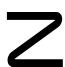
\includegraphics[keepaspectratio]{images/part001_3d6df7c1.jpg}}

因此，关系 \([M:L]=0\) 表示不存在同构于 L 的 M 的直因子子模。但这并不排除存在同构于 L 的 M 的子模；只需考虑例子 A=Z，L=Z/2Z，M=Z/4Z：Z-模 L 与 M 都是原始的且不同构，故 \([M:L]=0\)，而 L 同构于 M 的子模 \(2Z/4Z\)。

